\documentclass{standalone}
\usepackage{pgfplots}
\pgfplotsset{compat=newest}
\usepgfplotslibrary{patchplots}
\begin{document}
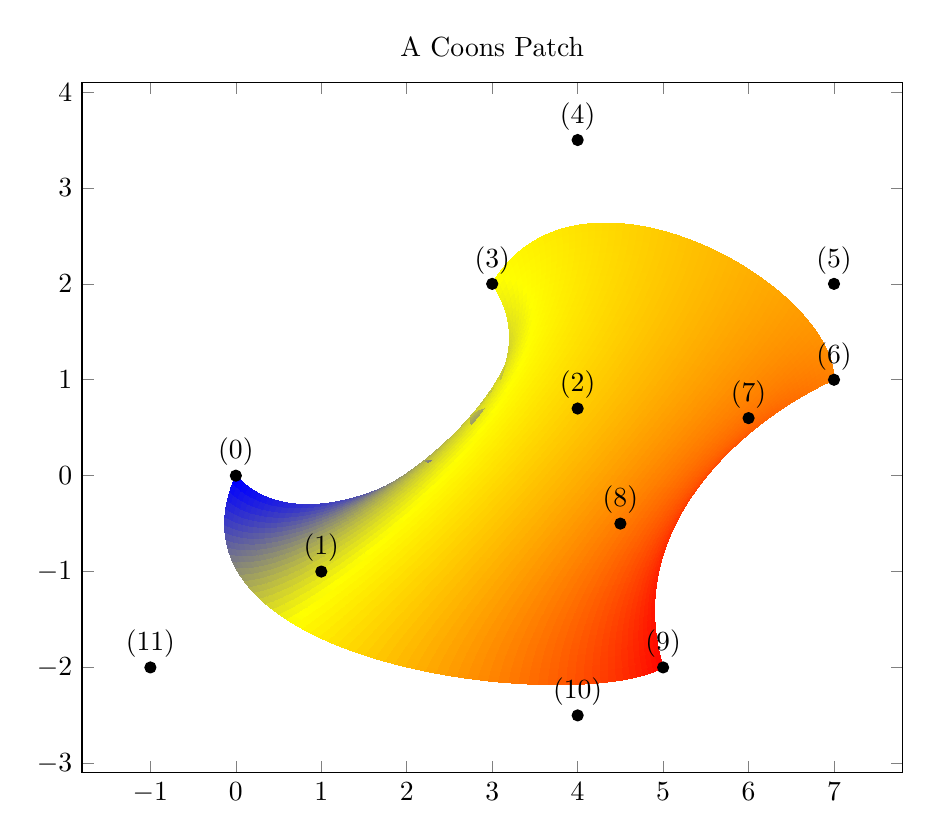
\begin{tikzpicture}
\begin{axis}[nodes near coords={(\coordindex)},
	width=12cm,
	title=A Coons Patch]
\addplot[mark=*,patch,patch type=coons,
	shader=interp,point meta=explicit] 
coordinates {
	(0,0)   [0] % first corner
	(1,-1)  [0] % Bezier control point between (0) and (3)
	(4,0.7) [0] % Bezier control point between (0) and (3)
	%
	(3,2)   [1] % second corner
	(4,3.5) [1] % Bezier control point between (3) and (6)
	(7,2)   [1] % Bezier control point between (3) and (6)
	%
	(7,1)      [2] % third corner
	(6,0.6)    [2] % Bezier control point between (6) and (9)
	(4.5,-0.5) [2] % Bezier control point between (6) and (9)
	%
	(5,-2)   [3] % fourth corner
	(4,-2.5) [3] % Bezier control point between (9) and (0)
	(-1,-2)  [3] % Bezier control point between (9) and (0)
};
\end{axis}
\end{tikzpicture}
\end{document}
